\documentclass[12pt,a4paper]{article}
\usepackage[utf8]{inputenc}
\usepackage[margin=1in]{geometry}
\usepackage{graphicx}
\usepackage{titlesec}
\usepackage{hyperref}
\usepackage{setspace}
\usepackage{float}

\titleformat{\section}{\normalfont\Large\bfseries}{\thesection}{1em}{}
\titleformat{\subsection}{\normalfont\large\bfseries}{\thesubsection}{1em}{}

\setlength{\parskip}{0.3em}

\begin{document}

% ==================== TITLE PAGE ====================
\begin{titlepage}
    \centering
    \vspace*{1cm}
    
    {\Large \textbf{INDIRA GANDHI NATIONAL OPEN UNIVERSITY}}\\[0.5cm]
    {\large School of Computer and Information Sciences}\\[0.3cm]
    {\large Maidan Garhi, New Delhi – 110068}\\[1.5cm]
    
    \rule{\textwidth}{1.5pt}\\[0.4cm]
    {\LARGE \textbf{MCSP - 232}}\\[0.3cm]
    {\Large \textbf{PROJECT SYNOPSIS}}\\[0.4cm]
    \rule{\textwidth}{1.5pt}\\[1.5cm]
    
    {\Large \textbf{AI-Based Real-Time eKYC System for Deepfake-Free Identity Verification}}\\[2.5cm]
    
    \begin{flushleft}
    {\large \textbf{Submitted by:}}\\[0.2cm]
    {\large Hardik Sharma}\\
    {\large Enrolment No: 2353777736}\\
    {\large Programme: MCA (MCAOL)}\\[1cm]
    
    {\large \textbf{Under the Guidance of:}}\\[0.2cm]
    {\large Anshul Sharma}\\
    {\large AI Engineer}\\
    {\large IDS Infotech Ltd. Chd.}\\[1.5cm]
    \end{flushleft}
    
    \vfill
    {\large \textbf{July 2025}}÷
    
\end{titlepage}

% ==================== CERTIFICATE ====================
\newpage
\thispagestyle{empty}

\begin{center}
    {\Large \textbf{CERTIFICATE OF ORIGINALITY}}
\end{center}

\vspace{1.5cm}

This is to certify that the project report entitled \textbf{``AI-Based Real-Time eKYC System for Deepfake-Free Identity Verification''} submitted to Indira Gandhi National Open University in partial fulfilment of the requirement for the award of the degree of \textbf{MASTER OF COMPUTER APPLICATIONS}, is an authentic and original work carried out by \textbf{Mr. Hardik Sharma} with enrolment no. \textbf{2353777736} under my guidance.

\vspace{0.8cm}

The matter embodied in this project is genuine work done by the student and has not been submitted whether to this University or to any other University / Institute for the fulfilment of the requirements of any course of study.

\vspace{2cm}

\begin{minipage}[t]{0.45\textwidth}
    \rule{6cm}{0.5pt}\\
    \textbf{Signature of the Student}\\[0.2cm]
    \textbf{Date:} \_\_\_\_\_\_\_\_\_\_\_\_\_\_\_\_\\[0.3cm]
    
    \textbf{Name:} Hardik Sharma\\
    \textbf{Enrolment No:} 2353777736
\end{minipage}
\hfill
\begin{minipage}[t]{0.45\textwidth}
    \rule{6cm}{0.5pt}\\
    \textbf{Signature of the Guide}\\[0.2cm]
    \textbf{Date:} \_\_\_\_\_\_\_\_\_\_\_\_\_\_\_\_\\[0.3cm]
    
    \textbf{Name:} Anshul Sharma\\
    \textbf{Designation:} AI Engineer\\
    \textbf{Organization:} IDS Infotech Ltd.
\end{minipage}

\newpage

% ==================== TABLE OF CONTENTS ====================
\tableofcontents
\newpage

\setstretch{1.15}

% ==================== SECTION 1: TITLE & INTRODUCTION ====================
\section{Title of the Project}

\textbf{AI-Based Real-Time eKYC System for Deepfake-Free Identity Verification}

\section{Introduction and Objectives}

\subsection{Introduction}

Digital transformation in banking has revolutionized customer onboarding through electronic Know Your Customer (eKYC) systems. However, sophisticated deepfake technology poses unprecedented security threats, with a 300\% increase in deepfake-based fraud attempts resulting in substantial financial losses. Current eKYC systems rely on static image matching and basic liveness detection, failing against GAN-generated faces, face-swap deepfakes, video replays, and morphed documents. RBI mandates robust multi-layered verification systems for real-time fraud detection. This project develops an AI-powered eKYC system integrating InsightFace for facial recognition, custom dual-stream neural network for deepfake detection with DinoV3 guidance, and video-based liveness analysis into a comprehensive platform performing multi-modal verification combining face matching, document OCR, and behavioral analysis with results in \textless\ 3 seconds while maintaining audit trails for regulatory compliance.

\begin{figure}[H]
\centering
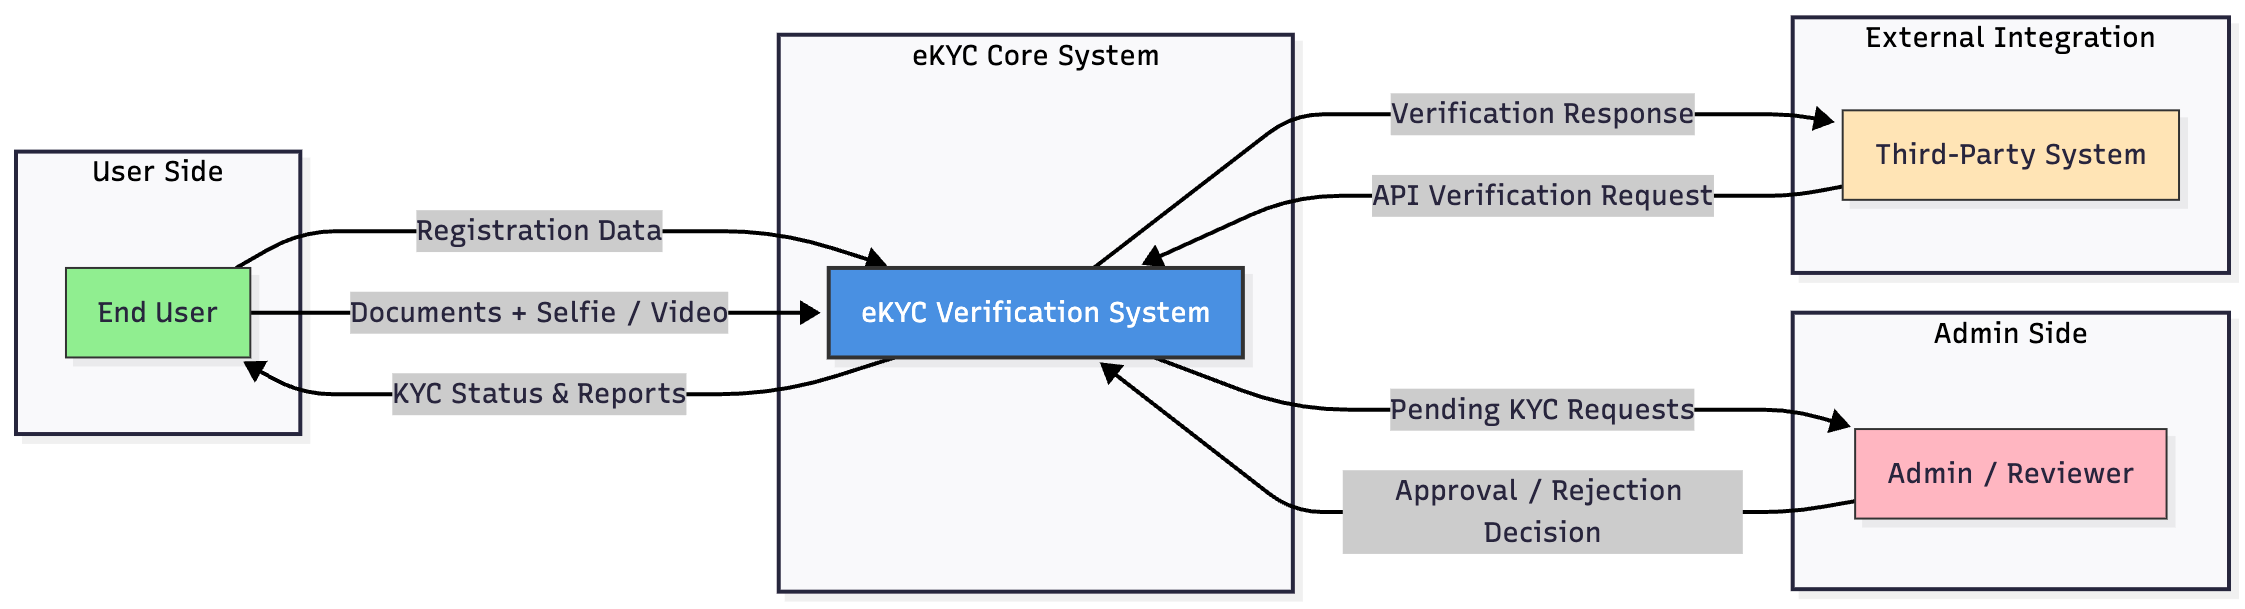
\includegraphics[width=1\textwidth]{main.png}
\caption{System Overview and Main Interface}
\end{figure}

\subsection{Objectives}

\textbf{Primary:} Design, develop, deploy comprehensive AI-powered eKYC system for secure real-time identity verification with deepfake detection.

\textbf{Specific Objectives:}
\begin{itemize}
    \item \textbf{Face Verification:} InsightFace Buffalo-S achieving 95\%+ accuracy matching ID photos with selfies via 512-dimensional embeddings
    \item \textbf{Deepfake Detection:} Dual-stream network (RGB + artifacts) with cross-attention fusion, DinoV3 guidance achieving 92\%+ detection accuracy
    \item \textbf{Liveness Detection:} Passive (texture analysis) and active (video blink/movement) verification with 3D face modeling preventing presentation attacks
    \item \textbf{Document Processing:} Support Aadhaar, PAN, Passport, DL, Voter ID with OCR extraction, validation, authenticity checks
    \item \textbf{System Development:} FastAPI backend, React TypeScript frontend, PostgreSQL+MongoDB databases, real-time processing \textless\ 3 seconds
    \item \textbf{Security:} TLS 1.3 encryption, JWT authentication, RBAC, AES-256 data encryption, OWASP Top 10 compliance
    \item \textbf{Compliance:} Audit trails, PDF reports, analytics dashboards meeting RBI KYC guidelines and data retention policies
\end{itemize}

\newpage

% ==================== SECTION 2: PROJECT CATEGORY ====================
\section{Project Category}

\textbf{Primary:} Artificial Intelligence, Machine Learning, Deep Learning

\textbf{Secondary:} Computer Vision, Image Processing, RDBMS + NoSQL, Web Development, Software Engineering, Data Science

\section{Tools, Platform, Hardware and Software Requirements}

\subsection{Software Requirements}

\textbf{Frontend:} React.js 18+ with TypeScript, HTML5, CSS3, Bootstrap 5, Axios, Chart.js

\textbf{Backend:} Python 3.10+, FastAPI, Uvicorn ASGI server, Pydantic validation, JWT authentication

\textbf{ML/DL:} PyTorch 2.0+, InsightFace (buffalo\_s), DinoV3, EfficientNet, EdgeNeXt, OpenCV 4.x, Albumentations, Tesseract/EasyOCR

\textbf{Database:} PostgreSQL 15+ (structured data), MongoDB 6+ (unstructured data)

\textbf{Libraries:} NumPy, Pandas, Pillow, Cryptography, WeasyPrint, pytest

\subsection{Hardware Requirements}

\textbf{Development:} Intel i5/AMD Ryzen 5+, 16 GB RAM (32 GB recommended), NVIDIA GPU 8GB+ VRAM or Colab T4, 500 GB SSD, Windows/Ubuntu/macOS

\textbf{Production:} Cloud server (AWS EC2/GCP), 8+ core CPU, 32 GB RAM, NVIDIA T4 GPU, 1 TB SSD, 100+ Mbps network

\textbf{Client:} Desktop/laptop/tablet/smartphone, Chrome 90+/Firefox 88+/Safari 14+/Edge 90+, 2MP camera minimum, 2 Mbps internet

\newpage

% ==================== SECTION 3: PROBLEM DEFINITION ====================
\section{Problem Definition, Requirements, Literature Review}

\subsection{Problem Definition}

Traditional eKYC faces critical vulnerabilities: inability detecting AI-generated faces from GANs, face-swap algorithms, morphing techniques; simple photo prints, video replays bypass basic liveness; manual review creates 2-5 day delays costing ₹50-200 per verification; single-modal verification lacks explainability, handles poor quality poorly, difficult integration.

\textbf{Problem:} Design AI-powered real-time eKYC system achieving 95\%+ identity accuracy, 92\%+ deepfake detection, liveness verification, \textless\ 3 seconds processing, multiple document OCR support, explainable decisions, audit trails, data security, 1000+ concurrent requests scaling, RESTful API integration.

\subsection{Functional Requirements}

The system provides secure user registration through OTP verification, JWT-based authentication, and profile management. It supports multiple identity documents (Aadhaar, PAN, Passport, Driving License, Voter ID) in JPEG/PNG/PDF formats under 10 MB, performing OCR extraction with validation and image quality checks. Face verification extracts and aligns faces, generates 512-dimensional InsightFace embeddings, and computes cosine similarity scores. Deepfake detection uses a dual-stream (RGB + frequency) model for images and videos, while liveness detection combines passive (texture) and active (blink, movement, 3D depth) methods. The decision engine auto-approves users when match $>$ 80\%, liveness $>$ 60\%, and deepfake $<$ 30\%, with limits on failed attempts. Admins can review flagged cases, approve or reject with remarks, and generate PDF reports with QR codes and analytics. RESTful APIs with key-based access, rate limiting, webhooks, and Swagger documentation enable smooth system integration.

\subsection{Non-Functional Requirements}

The platform achieves face verification in under 2 seconds and deepfake detection in under 3 seconds (images) or 10 seconds (videos), supporting over 100 concurrent requests with 95\% of queries completing within 100 ms. Security is ensured using HTTPS/TLS 1.3, bcrypt password hashing, AES-256 encryption, RBAC, and protection from SQL injection, XSS, and CSRF. Reliability is maintained through 99\% uptime, graceful error handling, automated daily backups, and data corruption prevention. The system is horizontally scalable to handle over 1 million users, 10 TB storage, and 10,000+ daily verifications. Compliance with RBI KYC (2023) and GDPR standards ensures 5-year data retention, secure deletion, and tamper-proof audit logs.

\subsection{Literature Review}

\textbf{Face Recognition:} Deng et al. (2019) introduced ArcFace with angular margin achieving 99.8\% accuracy. InsightFace provides pre-trained models balancing accuracy and speed, while Schroff et al. (2015) proposed FaceNet using triplet loss for embedding-based verification forming the core of our identity matching.

\textbf{Deepfake Detection:} Dual-stream architectures combining RGB and frequency-domain analysis significantly enhance detection. Chollet’s Xception (2017) with depthwise separable convolutions inspired EdgeNeXt; Hinton et al. (2015) introduced knowledge distillation applied in DinoV3; Durall et al. (2020) identified frequency artifacts in GAN-generated images using HPF/ELA.

\textbf{Liveness:} Boulkenafet et al. (2017) categorized liveness detection into passive and active methods. Our system employs both, combining texture-based and temporal consistency checks. Liu et al. (2018) demonstrated that depth cues and landmark consistency effectively distinguish live from spoofed faces.

\textbf{Compliance:} RBI Master Direction (2023) mandates V-CIP with liveness detection and secure record storage; our system is fully compliant.

\subsection{Project Planning and Scheduling}

\noindent\textbf{1.} A 6-month (24-week) plan includes Planning (1–3), Design (4–6), ML (6–12), Backend (13–16), Frontend (17–20), and Deployment (21–24).\\[4pt]
\textbf{2.} PERT Path: Requirements — Dataset Prep — Setup — Training — Features — Liveness — Testing — Integration — Security — Deployment.


\textbf{Gantt:} Overlapping phases for faster execution.

\begin{figure}[h]
\centering
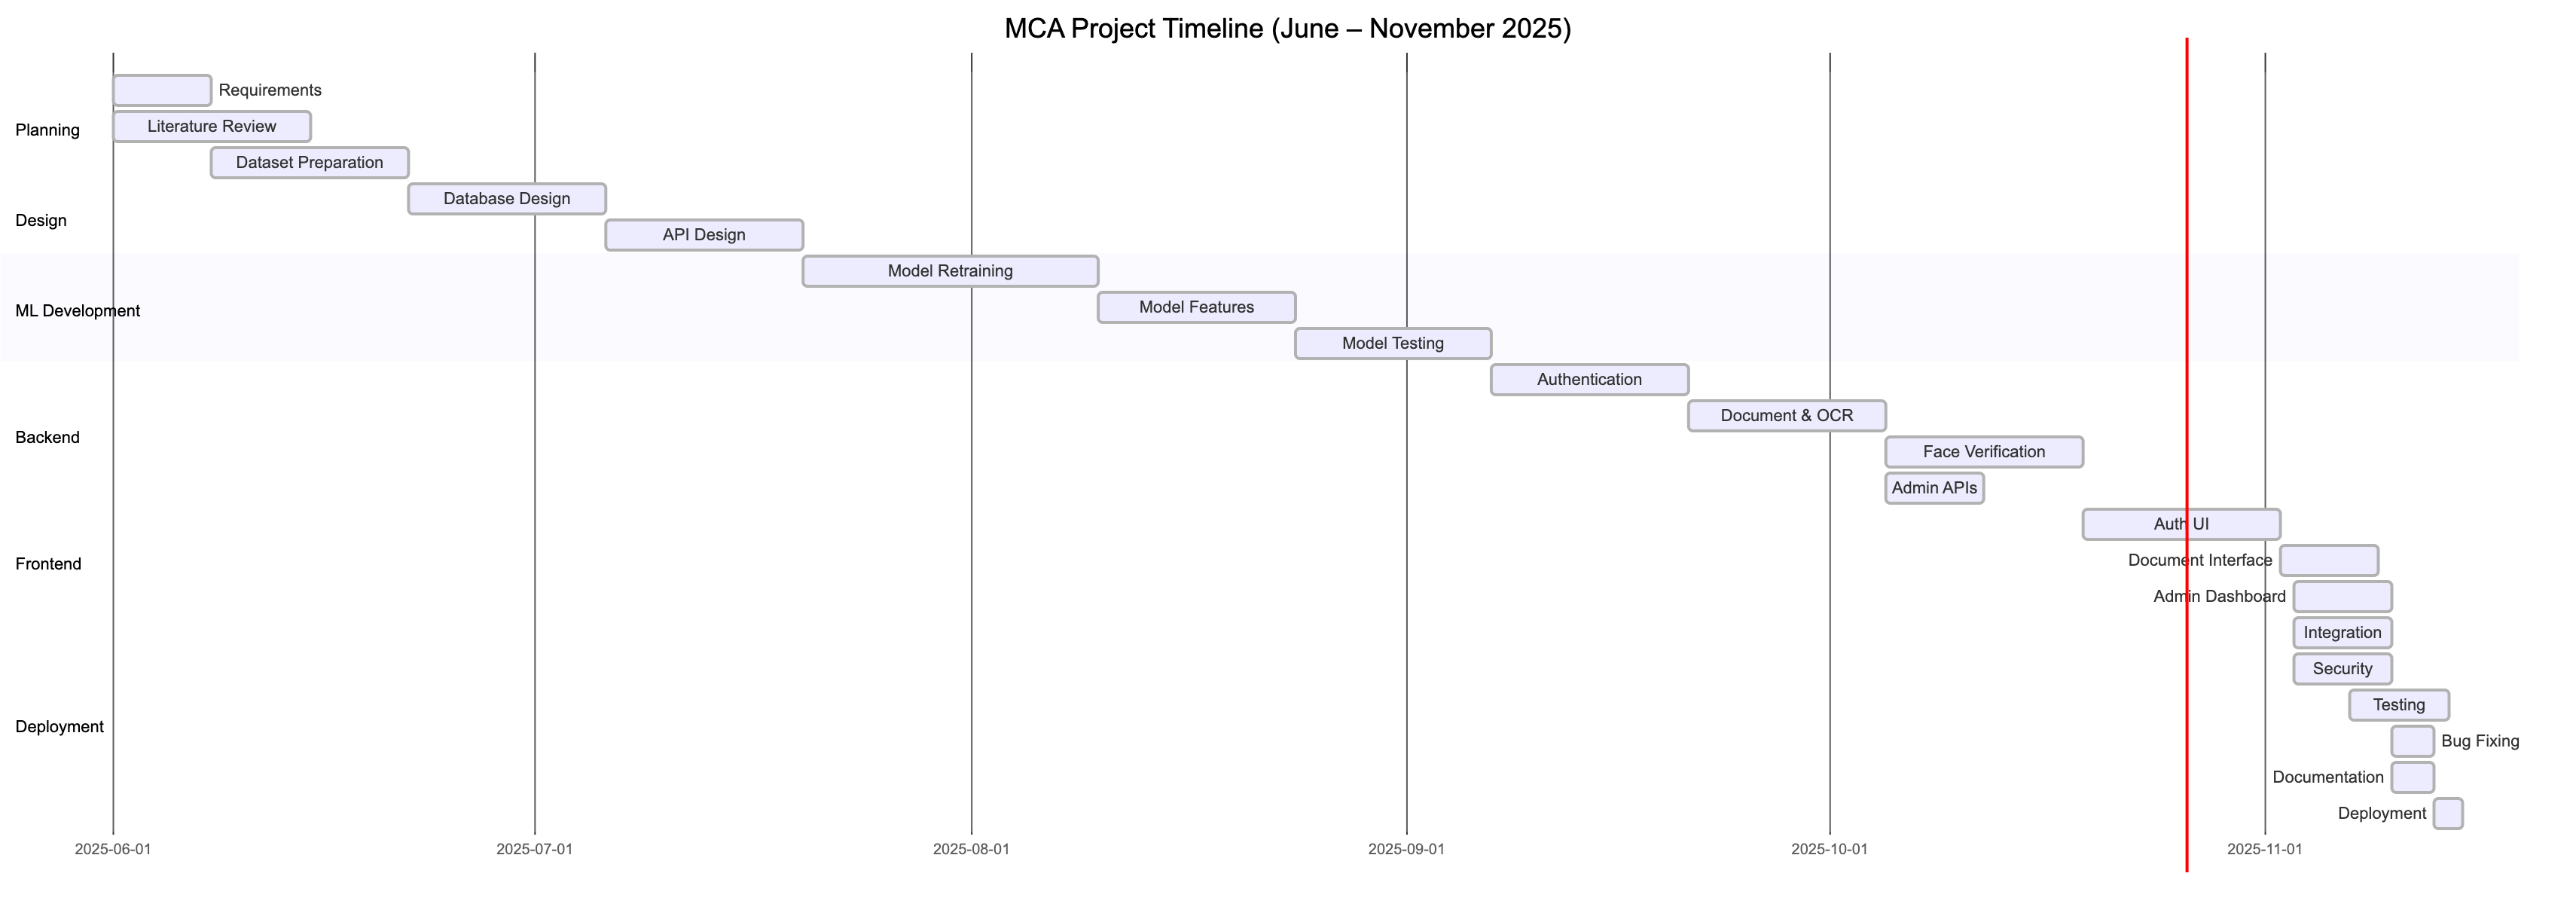
\includegraphics[width=\textwidth]{gantt_chart.png}
\caption{Gantt Chart showing project timeline.}
\end{figure}


\textbf{PERT Path:} Requirements → Dataset Prep → Setup → Training → Features → Liveness → Testing → Integration → Security → Deployment.

\begin{figure}[H]
\centering
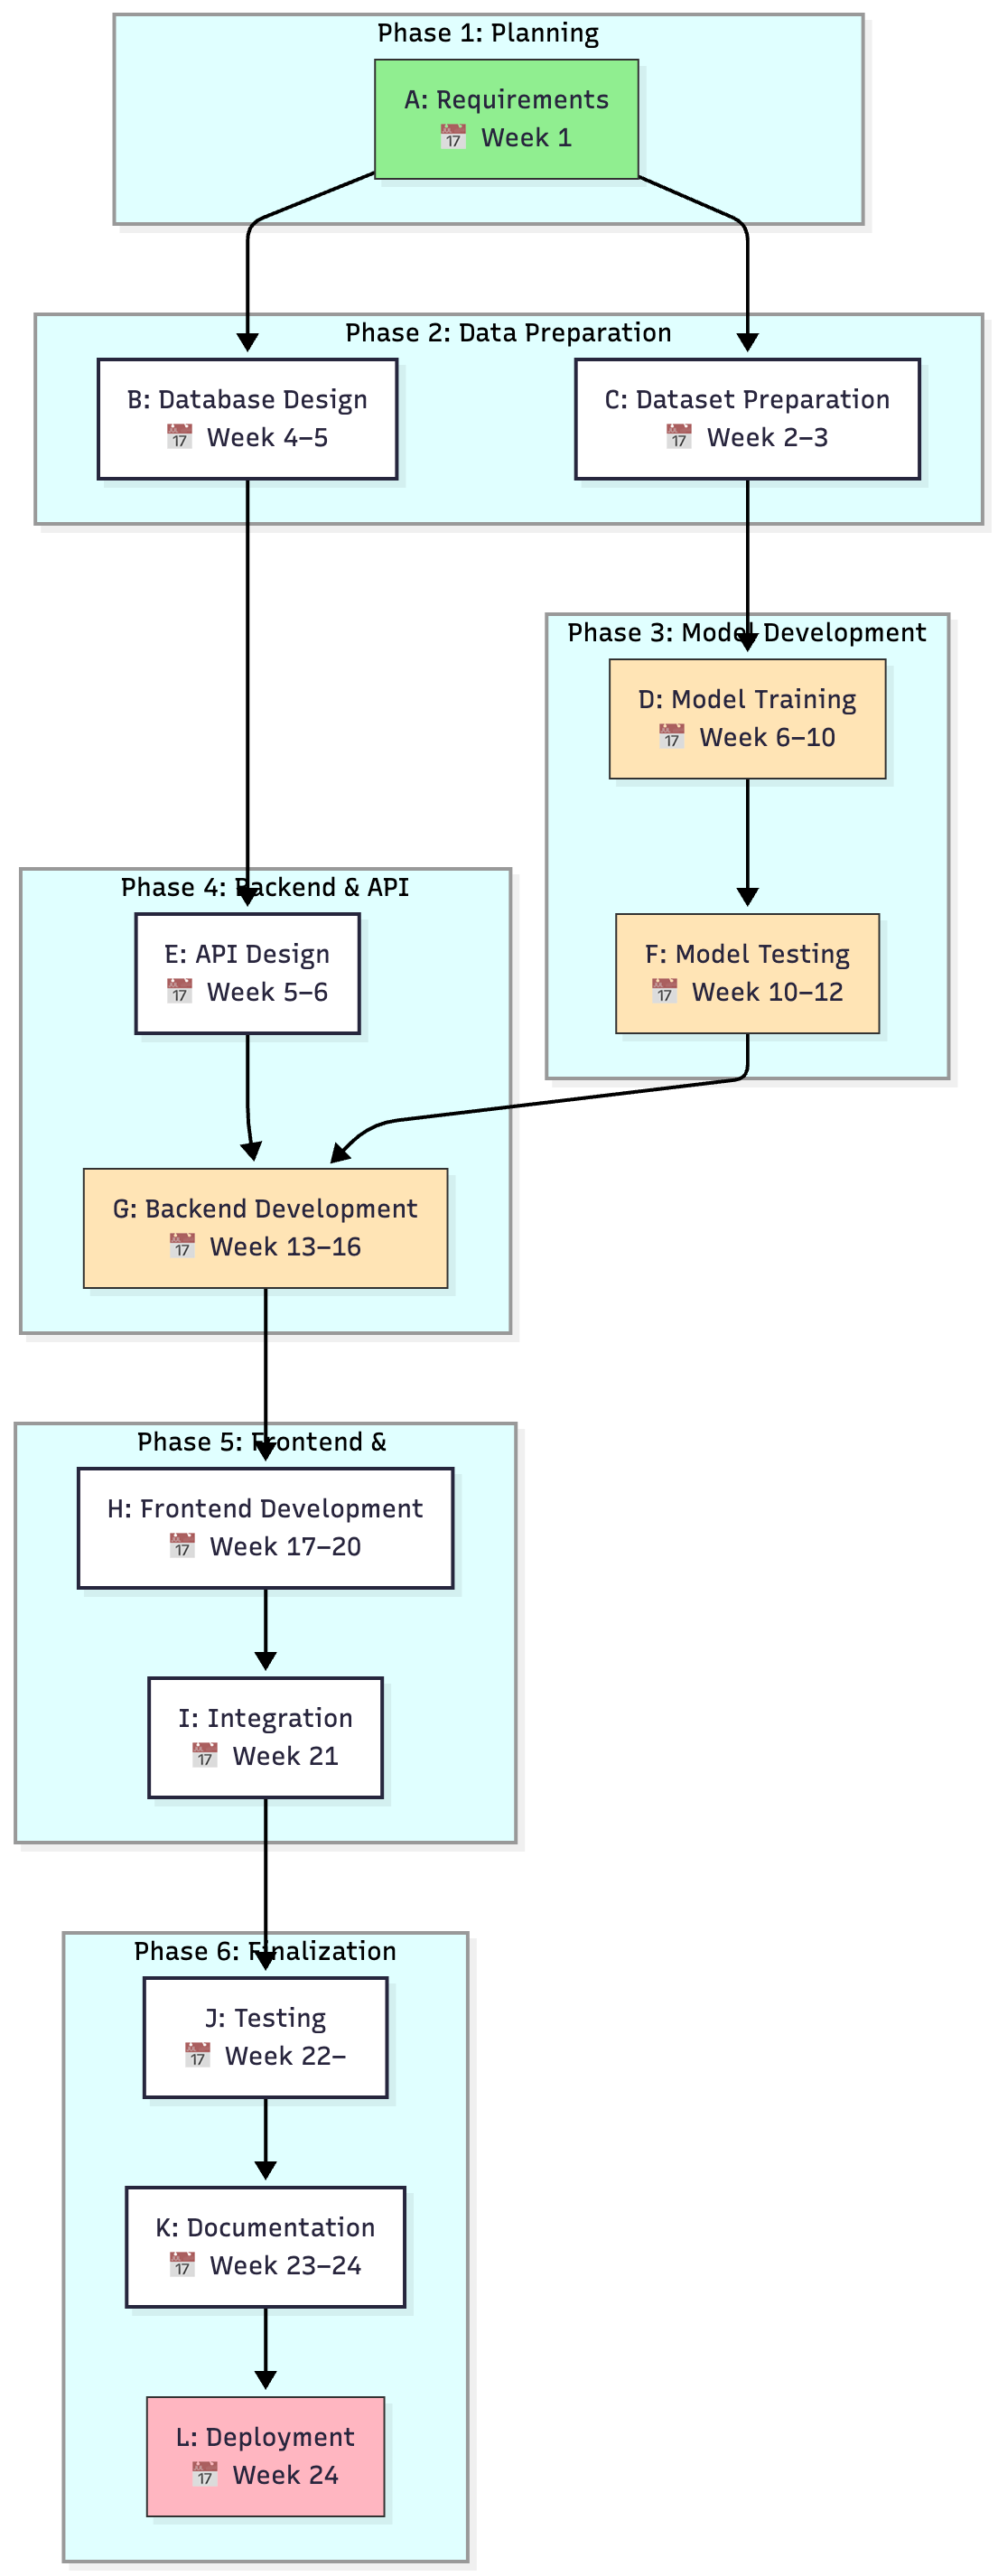
\includegraphics[width=0.6\textwidth]{pert_chart.png}
\caption{PERT Chart showing key tasks and dependencies.}
\end{figure}

% ==================== SECTION 4: SCOPE ====================
\section{Scope of the Solution}

\subsection{In Scope}

User registration and authentication, profile management; upload and processing of Aadhaar, PAN, Passport, DL, Voter ID, Bank Statement, and Utility Bill; OCR extraction with validation; face detection, alignment, and embedding generation; face matching between ID and selfie; deepfake detection via dual-stream network; passive and active liveness detection; frame-by-frame video analysis; automated decision engine with configurable thresholds; manual review queue for flagged cases; admin dashboard with analytics; PDF report generation with QR codes; audit trails and compliance logging; RESTful API integration; end-to-end security (encryption, RBAC, input validation); responsive web interface.

\subsection{Out of Scope}

Mobile native applications (iOS/Android); blockchain integration; real-time video streaming; multilingual support beyond English; fingerprint or iris biometrics; direct UIDAI API integration; payment gateway support; voice deepfake detection; offline edge deployment (reserved for future enhancement).

% \newpage

% ==================== SECTION 5: ANALYSIS ====================
\section{System Analysis}

System analysis models information flow through Data Flow Diagrams between processes, data stores, external entities.

\subsection{Data Flow Diagrams}

\textbf{DFD Level 0:} eKYC System interacts with End User (provides registration, documents, selfie/video; receives status, reports), Admin (receives pending requests; provides decisions), Third-Party (sends API requests; receives responses).
\newpage
\textbf{DFD Level 1 Processes:}

\begin{figure}[H]
\centering
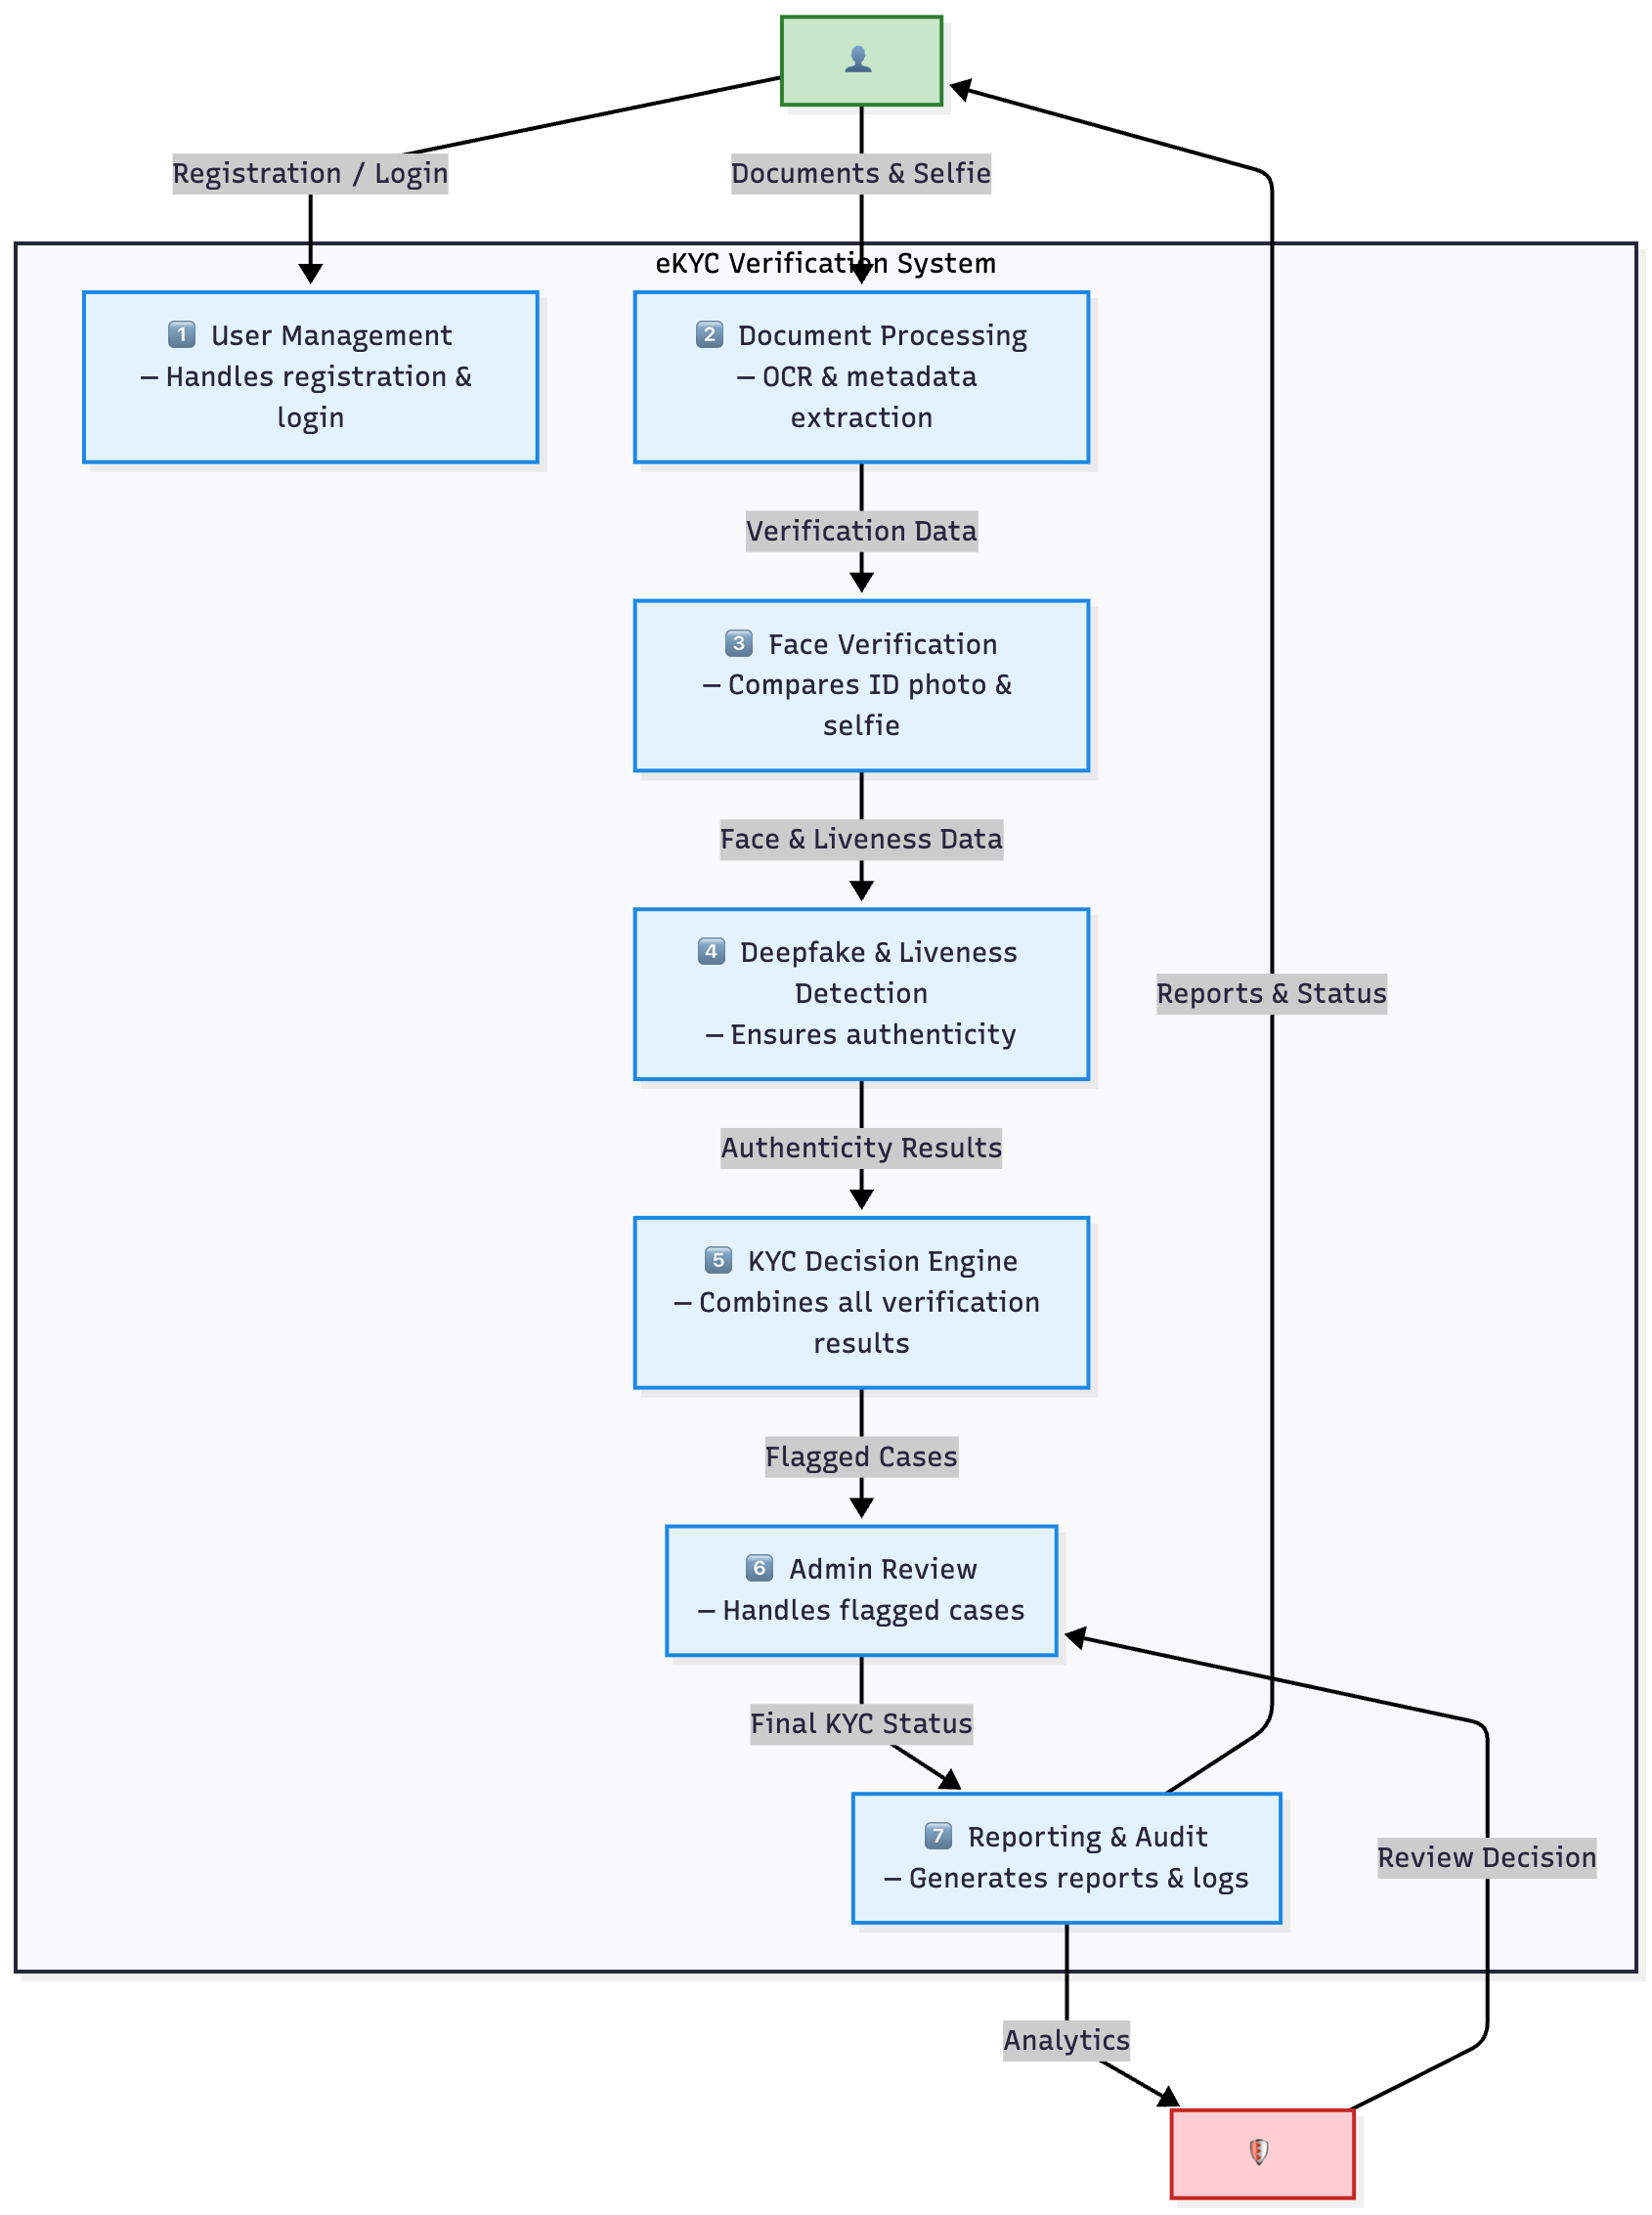
\includegraphics[width=\textwidth]{dfd_l1.png}
\caption{DFD Level 1 decomposing system into seven major processes}
\end{figure}

\textbf{1.0-User Management:} Registration, authentication, profiles. In: registration info, credentials. Out: profile, JWT. Store: Users DB.

\textbf{2.0-Document Processing:} Upload, OCR extraction, validation. In: document images. Out: metadata, OCR data. External: OCR Engine. Store: Documents DB.

\textbf{3.0-Face Verification:} Face detection, alignment, embeddings, similarity. In: ID photo, selfie. Out: match score, embeddings. External: InsightFace. Store: Sessions DB.

\textbf{4.0-Deepfake \& Liveness:} Artifact analysis, temporal checks. In: selfie, video frames. Out: authenticity, liveness score. External: Deepfake Model. Store: Video Frames DB.

\textbf{5.0-Decision Engine:} Score aggregation, threshold comparison, auto-decision. In: match, deepfake, liveness scores. Out: KYC status. Store: Sessions DB.

\textbf{6.0-Admin Review:} Present flagged cases, record decisions. In: flagged cases, decisions. Out: approval/rejection. Store: Reviews DB.

\textbf{7.0-Reporting:} PDF reports, analytics, compliance logs. In: session data, activity. Out: reports, analytics. Store: Audit DB.

\textbf{DFD Level 2 (Face Verification):} 3.1-Face Detection \& Alignment (detects regions, 68 landmarks, aligns); 3.2-Extract ID Embedding (InsightFace 512-dim); 3.3-Extract Selfie Embedding; 3.4-Calculate Match Score (cosine similarity 0-100\%); 3.5-Store Results (encrypted embeddings, scores, timestamp).

\subsection{Activity Diagram Workflow}

User registers → verifies OTP → logs in → uploads document → OCR extraction (retry if fails) → uploads selfie → quality check (retry if fails) → face verification → deepfake detection → liveness check → score calculation → auto-decision (approve if thresholds met; else flag for review) → admin reviews (approve/reject/reupload) → user notified → complete.

% \newpage

% ==================== SECTION 6: DATABASE DESIGN ====================
\section{Database Design}

\subsection{Entity Relationship Diagram}

\begin{figure}[H]
\centering
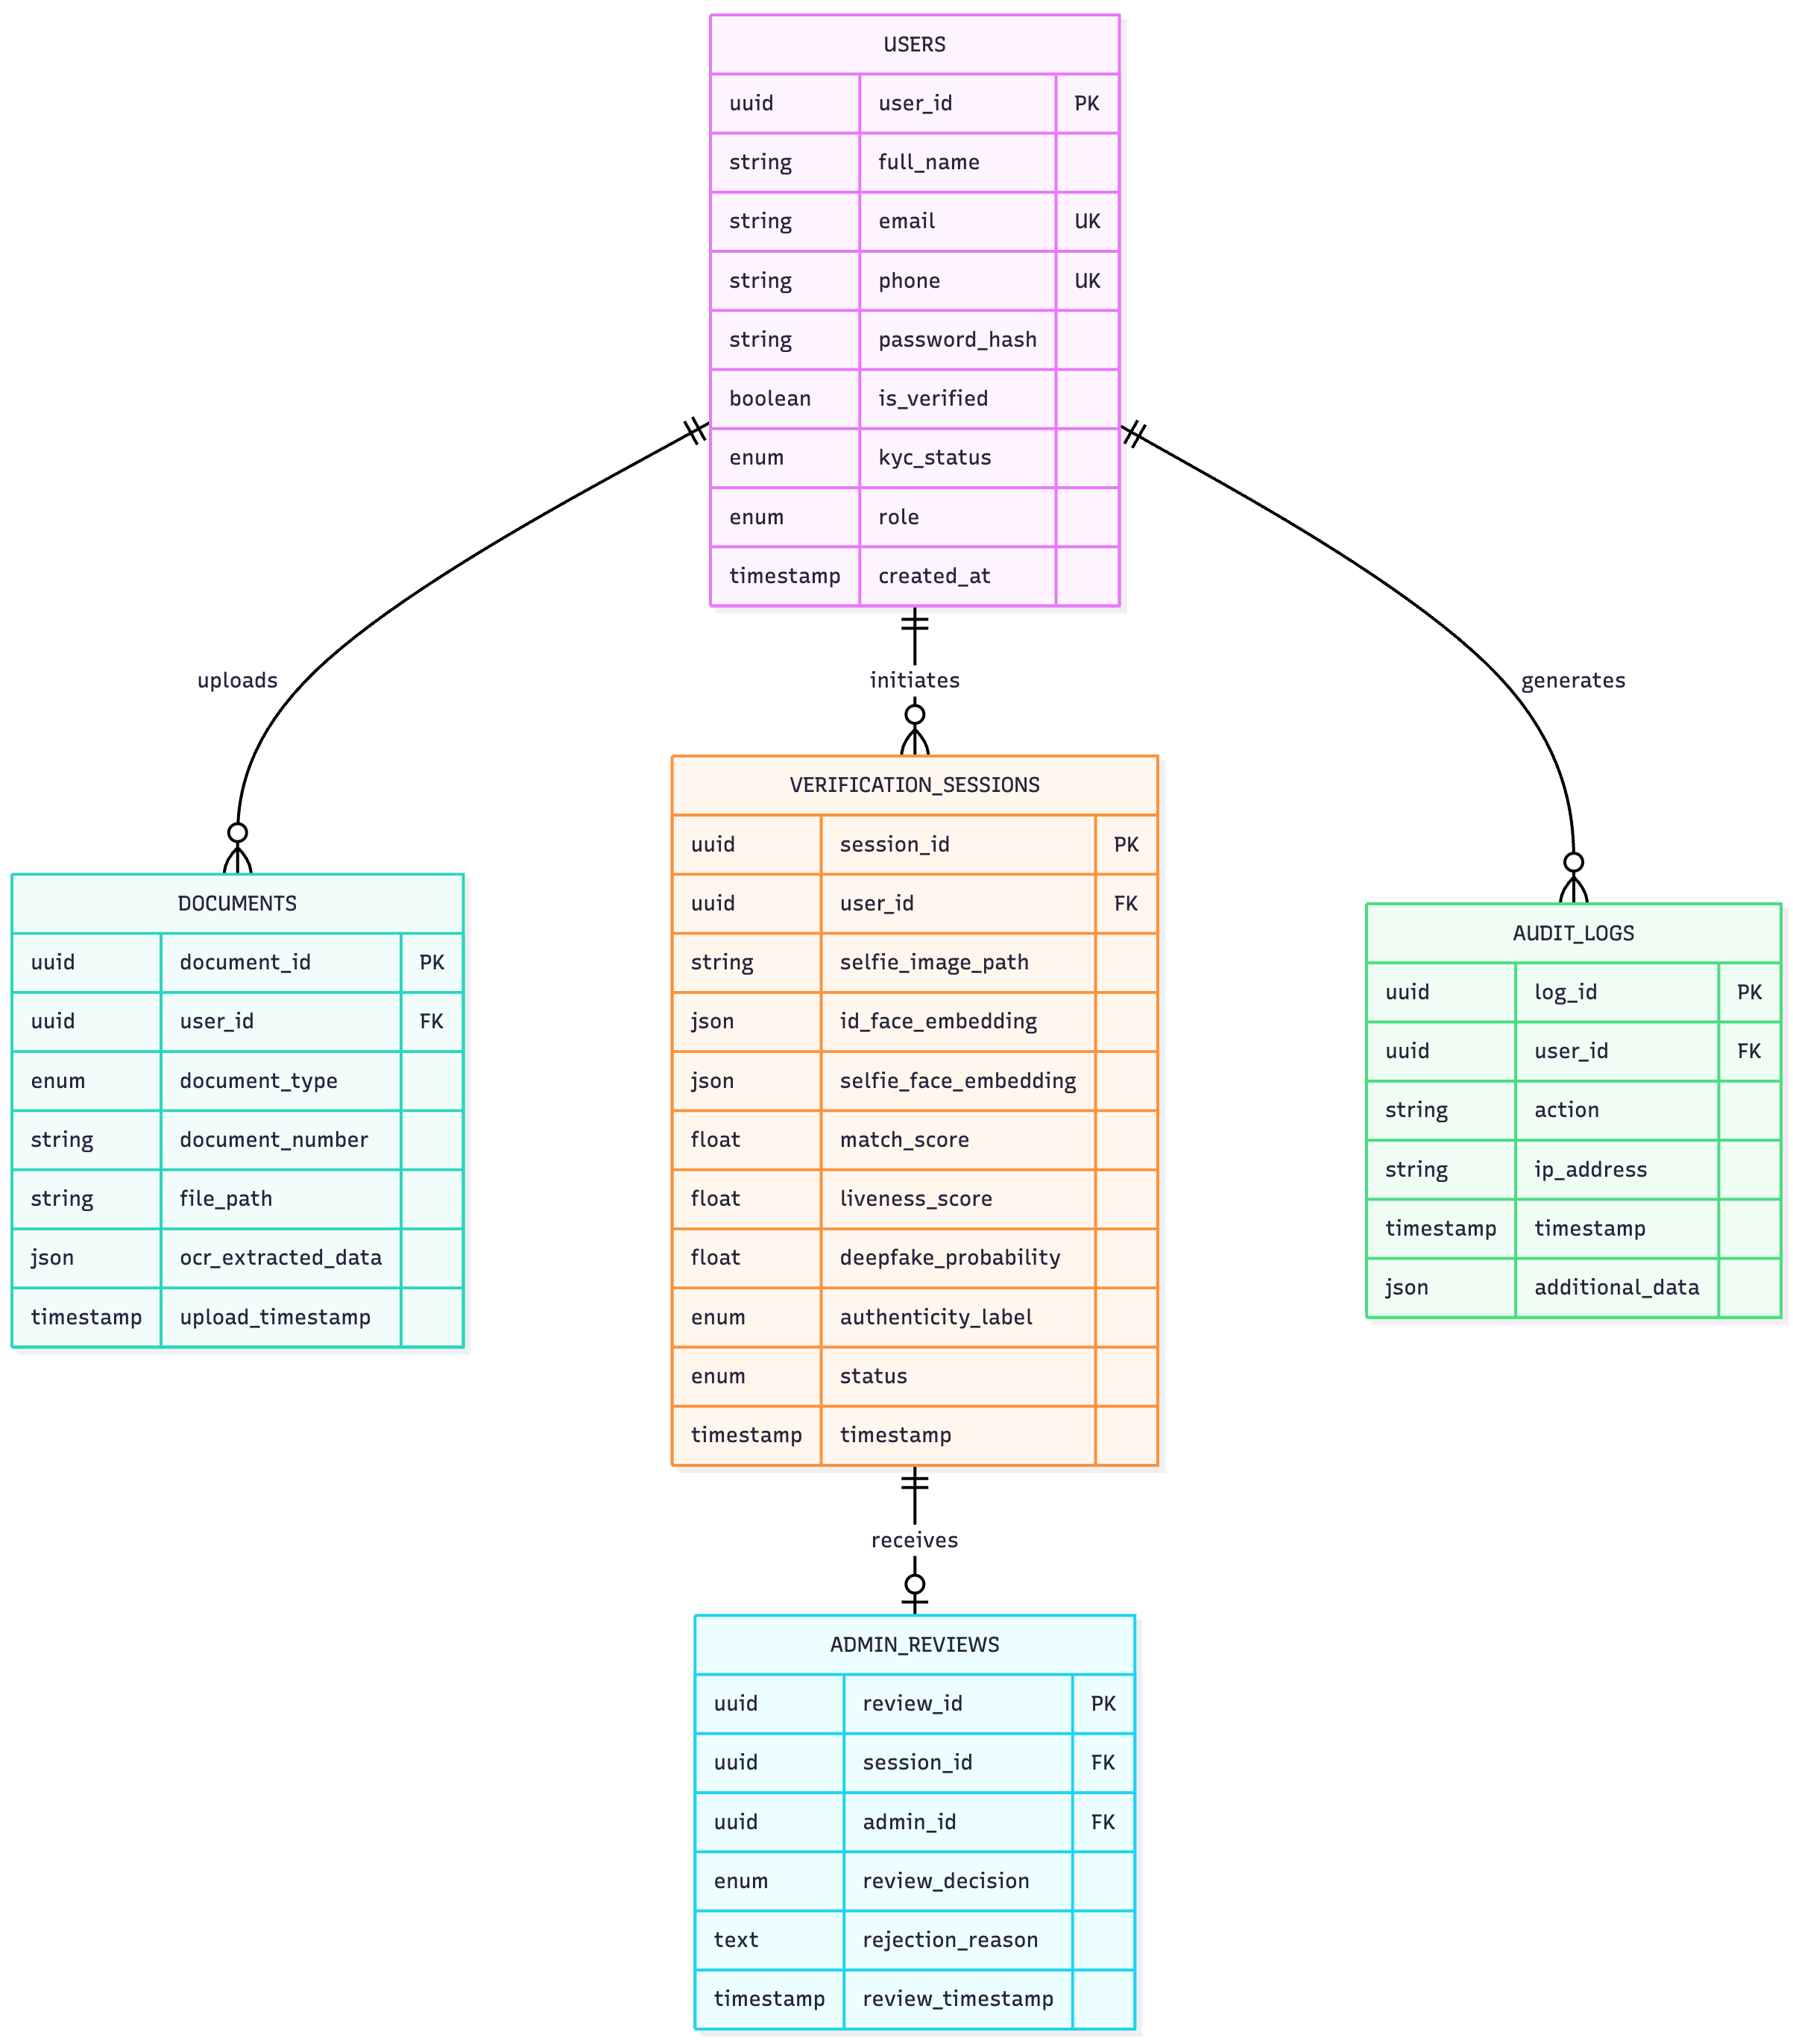
\includegraphics[width=\textwidth]{er_diagram.png}
\caption{ER Diagram showing entities, relationships, and cardinality}
\end{figure}

\textbf{Relationships:} USERS (1) → (M) DOCUMENTS, USERS (1) → (M) VERIFICATION\_SESSIONS, VERIFICATION\_SESSIONS (1) → (M) VIDEO\_FRAMES, VERIFICATION\_SESSIONS (1) → (1) ADMIN\_REVIEWS, USERS-Admin (1) → (M) ADMIN\_REVIEWS, USERS (1) → (M) AUDIT\_LOGS.

\subsection{Database Tables}

\subsubsection{Table 1: USERS}
\begin{verbatim}
CREATE TABLE users (
    user_id UUID PRIMARY KEY,
    full_name VARCHAR(255) NOT NULL,
    email VARCHAR(255) UNIQUE NOT NULL,
    phone VARCHAR(15) UNIQUE NOT NULL,
    password_hash VARCHAR(255) NOT NULL,
    is_verified BOOLEAN DEFAULT FALSE,
    kyc_status ENUM('pending','approved','rejected','under_review') 
               DEFAULT 'pending',
    role ENUM('user','admin','reviewer') DEFAULT 'user',
    created_at TIMESTAMP DEFAULT CURRENT_TIMESTAMP,
    updated_at TIMESTAMP DEFAULT CURRENT_TIMESTAMP
);
\end{verbatim}
\textbf{Constraints:} PK (user\_id), UNIQUE (email, phone), NOT NULL (name, email, phone, password\_hash), CHECK (kyc\_status, role IN valid enums).

\subsubsection{Table 2: DOCUMENTS}
\begin{verbatim}
CREATE TABLE documents (
    document_id UUID PRIMARY KEY,
    user_id UUID NOT NULL,
    document_type ENUM('aadhaar','pan','passport','driving_license',
                       'voter_id','bank_statement','utility_bill'),
    document_number VARCHAR(50),
    file_path VARCHAR(500) NOT NULL,
    ocr_extracted_data JSON,
    upload_timestamp TIMESTAMP DEFAULT CURRENT_TIMESTAMP,
    is_verified BOOLEAN DEFAULT FALSE,
    FOREIGN KEY (user_id) REFERENCES users(user_id) ON DELETE CASCADE
);
\end{verbatim}
\textbf{Constraints:} PK (document\_id), FK (user\_id→users CASCADE), CHECK (document\_type IN valid enum), NOT NULL (user\_id, file\_path).

\subsubsection{Table 3: VERIFICATION\_SESSIONS}
\begin{verbatim}
CREATE TABLE verification_sessions (
    session_id UUID PRIMARY KEY,
    user_id UUID NOT NULL,
    selfie_image_path VARCHAR(500) NOT NULL,
    video_path VARCHAR(500),
    id_face_embedding JSON,
    selfie_face_embedding JSON,
    match_score FLOAT CHECK (match_score BETWEEN 0 AND 100),
    liveness_score FLOAT CHECK (liveness_score BETWEEN 0 AND 100),
    deepfake_probability FLOAT CHECK (deepfake_probability 
                                      BETWEEN 0 AND 100),
    authenticity_label ENUM('real','fake'),
    quality_checks JSON,
    timestamp TIMESTAMP DEFAULT CURRENT_TIMESTAMP,
    status ENUM('pending','approved','rejected','flagged') 
           DEFAULT 'pending',
    admin_reviewed BOOLEAN DEFAULT FALSE,
    FOREIGN KEY (user_id) REFERENCES users(user_id) ON DELETE CASCADE
);
\end{verbatim}
\textbf{Constraints:} PK (session\_id), FK (user\_id→users CASCADE), CHECK (scores 0-100 range), NOT NULL (user\_id, selfie\_image\_path).

\subsubsection{Table 4: ADMIN\_REVIEWS}
\begin{verbatim}
CREATE TABLE admin_reviews (
    review_id UUID PRIMARY KEY,
    session_id UUID NOT NULL,
    admin_id UUID NOT NULL,
    review_decision ENUM('approved','rejected','request_reupload'),
    rejection_reason TEXT,
    review_timestamp TIMESTAMP DEFAULT CURRENT_TIMESTAMP,
    FOREIGN KEY (session_id) REFERENCES verification_sessions(session_id)
                ON DELETE CASCADE,
    FOREIGN KEY (admin_id) REFERENCES users(user_id) ON DELETE SET NULL,
    CHECK (review_decision != 'rejected' OR rejection_reason IS NOT NULL)
);
\end{verbatim}
\textbf{Constraints:} PK (review\_id), FKs (session\_id→sessions CASCADE, admin\_id→users SET NULL), CHECK (rejected requires reason).

\subsubsection{Table 5: AUDIT\_LOGS}
\begin{verbatim}
CREATE TABLE audit_logs (
    log_id UUID PRIMARY KEY,
    user_id UUID,
    action VARCHAR(100) NOT NULL,
    ip_address VARCHAR(45),
    user_agent TEXT,
    timestamp TIMESTAMP DEFAULT CURRENT_TIMESTAMP,
    additional_data JSON,
    FOREIGN KEY (user_id) REFERENCES users(user_id) ON DELETE SET NULL
);
CREATE INDEX idx_audit_timestamp ON audit_logs(timestamp);
CREATE INDEX idx_audit_user ON audit_logs(user_id);
\end{verbatim}
\textbf{Constraints:} PK (log\_id), FK (user\_id→users SET NULL), NOT NULL (action), Indexes (timestamp, user\_id for fast queries).

\subsection{Normalization}

\textbf{1NF:} All attributes atomic, no multi-valued attributes, no repeating groups, primary keys defined.

\textbf{2NF:} In 1NF, all non-key attributes fully dependent on primary key, no partial dependencies, no composite keys.

\textbf{3NF:} In 2NF, no transitive dependencies, non-key attributes depend only on primary key. Admin info stored in USERS (referenced by admin\_id), not duplicated in ADMIN\_REVIEWS.

\textbf{Denormalization:} VERIFICATION\_SESSIONS stores embeddings directly (avoids JOIN); JSON fields (ocr\_data, quality\_checks) allow document format flexibility.

% \newpage

% ==================== SECTION 7: MODULE STRUCTURE ====================
\section{Module Structure and Implementation}

The system is divided into three core modules handling document processing, face verification, and KYC decision workflow.

\subsection{Module 1: Document Processing and OCR}

\begin{itemize}
    \item \textbf{Purpose:} Handles document upload, text extraction, and validation.
    \item \textbf{Sub-Components:} 
    \begin{itemize}
        \item \textbf{Upload Handler:} Validates file type/size, assigns UUID filename, stores under \texttt{/storage/user\_id/}.
        \item \textbf{OCR Engine:} Preprocesses input and performs text extraction using Tesseract OCR for Aadhaar, PAN, Passport.
        \item \textbf{Validator:} Verifies Aadhaar/PAN formats via regex and stores results as JSON.
    \end{itemize}
    \item \textbf{Data Structure:}
\begin{verbatim}
class DocumentProcessor:
    document_id, user_id, file_path, ocr_data, validation_status
\end{verbatim}
    \item \textbf{Process Logic:} 
\begin{verbatim}
process_document(user_id, doc_type, file):
    validate(file)
    ocr_data = tesseract.extract(file)
    if not valid: return error
    save_to_db(user_id, doc_type, ocr_data)
\end{verbatim}
\end{itemize}

\subsection{Module 2: Face Verification and Deepfake Detection}

\begin{itemize}
    \item \textbf{Purpose:} Performs face matching and fake content detection.
    \item \textbf{Sub-Components:} 
    \begin{itemize}
        \item \textbf{Face Verification:} Uses RetinaFace + InsightFace (Buffalo-S), generates 512-d embeddings, cosine similarity ≥80\% threshold.
        \item \textbf{Deepfake Detection:} Dual-stream EfficientNet-B0 + EdgeNeXt fusion with cross-attention; outputs real/fake score (0–100\%).
        \item \textbf{Video Analysis:} Extracts 2 FPS frames, checks temporal consistency, averages scores.
    \end{itemize}
    \item \textbf{Data Structure:}
\begin{verbatim}
class FaceVerifier:
    session_id, id_emb, selfie_emb, match_score, df_prob, authenticity
\end{verbatim}
    \item \textbf{Process Logic:}
\begin{verbatim}
verify_and_detect(id_path, selfie_path):
    match_score = cosine(id_emb, selfie_emb)
    df_prob = model.predict(selfie)
    authenticity = "FAKE" if df_prob>50 else "REAL"
\end{verbatim}
\end{itemize}

\subsection{Module 3: KYC Decision and Admin Review}

\begin{itemize}
    \item \textbf{Purpose:} Aggregates scores and finalizes automated or manual KYC decisions.
    \item \textbf{Sub-Components:}
    \begin{itemize}
        \item \textbf{Decision Engine:} Auto-approves if match≥80\%, liveness≥60\%, deepfake≤30\%; otherwise flags.
        \item \textbf{Admin Review:} Displays pending cases; admin can approve, reject, or request reupload.
        \item \textbf{Notification:} Sends alerts via email/SMS (SMTP/Twilio) and logs all actions.
    \end{itemize}
    \item \textbf{Data Structure:}
\begin{verbatim}
class DecisionEngine:
    session_id, thresholds, decision_status, flag_reasons
\end{verbatim}
    \item \textbf{Process Logic:}
\begin{verbatim}
make_decision(session_id):
    if match>=80 and df_prob<=30: approve()
    else: flag_and_notify_admin()
\end{verbatim}
\end{itemize}

\subsection{Implementation Methodology}

\begin{itemize}
    \item \textbf{Development:} Agile 2-week sprints, modular RESTful API design, and test-driven development.
    \item \textbf{Deployment:} Docker-based setup (Compose for local, AWS/GCP for cloud), NGINX reverse proxy, CI/CD via GitHub Actions.
\end{itemize}

\subsection{Reports Generated}

\begin{itemize}
    \item \textbf{KYC Report:} User details, document info, scores, final status, and QR-verified verification ID.
    \item \textbf{Admin Report:} Session details, AI scores, admin decisions, timestamps.
    \item \textbf{Analytics Dashboard:} Statistics on approvals, rejections, deepfake trends, processing time.
    \item \textbf{Audit Trail:} Logs user/admin activity, API calls, failed attempts, and security events.
    \item \textbf{Compliance Report:} Aggregated verification stats, manual reviews, incidents, and uptime metrics.
\end{itemize}

% \newpage

% ==================== SECTION 8: NETWORK ARCHITECTURE ====================
\section{Overall Network Architecture}

The system follows a secure three-tier client-server architecture integrated with ML inference and external services.

\begin{itemize}
    \item \textbf{Presentation Tier:} React.js single-page application (SPA) served via NGINX with HTTPS REST APIs; responsive across devices and major browsers.
    \item \textbf{Application Tier:} FastAPI backend running on Uvicorn ASGI with JWT-based authentication, async request handling, containerized deployment, and load balancing (NGINX/AWS ALB).
    \item \textbf{Data Tier:} PostgreSQL for structured data (users, documents, sessions), MongoDB for semi-structured logs, Redis cache for sessions, daily backups to isolated storage.
    \item \textbf{ML Inference Layer:} PyTorch models preloaded at startup; GPU-accelerated inference (NVIDIA T4); batch processing and model versioning supported.
    \item \textbf{External Services:} Twilio/AWS SNS for SMS, Gmail API/SendGrid for emails, AWS S3 for document storage.
    \item \textbf{Security Layer:} TLS 1.3 encryption for all traffic, firewall allowing only ports 80/443, middleware-based rate limiting, and Web Application Firewall (WAF) for OWASP protection.
\end{itemize}


% ==================== SECTION 9: SECURITY ====================
\section{Implementation of Security Mechanisms}

Security is implemented at multiple layers following the principles of defense-in-depth to ensure data protection, secure authentication, and overall system resilience.

\subsection{Authentication and Authorization}

\begin{itemize}
    \item \textbf{JWT Authentication:} Tokens are issued upon login containing \texttt{user\_id}, \texttt{role}, \texttt{issued\_at}, and \texttt{expires\_at}. They have a 24-hour expiry with refresh capability, stored in HTTP-only cookies (not \texttt{localStorage}), and verified on every API request.
    \item \textbf{RBAC (Role-Based Access Control):} Three roles are defined — \textit{User} (upload documents, view own status), \textit{Reviewer} (view pending, approve/reject), and \textit{Admin} (all reviewer permissions plus analytics, audit logs, and configuration). A permission matrix is enforced at the API level, and unauthorized requests return HTTP 403.
\end{itemize}

\subsection{Password Security}

\begin{itemize}
    \item \textbf{Hashing:} Passwords are hashed using the \texttt{bcrypt} algorithm with a cost factor of 12 and automatically generated salt, providing resistance against rainbow table and timing attacks.
    \item \textbf{Policy:} Passwords must be at least 8 characters long, contain uppercase, lowercase, digit, and special characters, and are checked against common dictionaries. Reuse of the last three passwords is not permitted.
\end{itemize}

\subsection{Data Encryption}

\begin{itemize}
    \item \textbf{At Rest:} AES-256 encryption is applied to sensitive fields (embeddings, document numbers, phone numbers). Keys are stored in environment variables (never hardcoded) with a 90-day rotation policy. Uploaded documents are encrypted before storage.
    \item \textbf{In Transit:} All communications occur over HTTPS (TLS 1.3) with SSL certificates from trusted CAs (e.g., Let’s Encrypt). HTTP Strict Transport Security (HSTS) and Perfect Forward Secrecy (PFS) are enabled.
\end{itemize}

\subsection{Input Validation}

\begin{itemize}
    \item \textbf{Frontend:} Client-side checks include email format regex, 10-digit phone number validation, supported file types (JPEG/PNG/PDF), file size below 10MB, and real-time password strength indicators.
    \item \textbf{Backend:} Server-side validation uses Pydantic for request validation, parameterized SQL queries to prevent injection, HTML escaping to prevent XSS, and protection against path traversal and command injection. All inputs are validated before processing.
\end{itemize}

\subsection{API Security}

\begin{itemize}
    \item \textbf{Rate Limiting:} User endpoints are limited to 100 requests/hour, API keys to 1000 requests/hour, login attempts to 5 failures per 15 minutes (to prevent brute force), and document uploads to 10/hour.
    \item \textbf{API Key Management:} Keys are 32-character random strings hashed with \texttt{bcrypt}, linked to organizations with rate limits, support instant revocation, and have enforced expiration dates.
\end{itemize}

\subsection{File Upload Security}

\begin{itemize}
    \item \textbf{Validation:} Files undergo MIME type and magic byte verification, 10MB size restriction, filename sanitization (removal of special characters), and optional virus scanning using ClamAV.
    \item \textbf{Storage:} Files are stored outside the web root with randomized UUID filenames, no direct URL access, served only via authenticated endpoints, and stored in isolated directories per user.
\end{itemize}

\subsection{Attack Protection}

\begin{itemize}
    \item \textbf{SQL Injection:} Prevented using parameterized queries and ORM-safe methods (SQLAlchemy).
    \item \textbf{XSS:} Mitigated through HTML escaping, CSP headers, and HTTP-only cookies.
    \item \textbf{CSRF:} Protected using CSRF tokens for all state-changing operations, the SameSite cookie attribute, and the double-submit cookie pattern.
\end{itemize}

\subsection{Audit Logging}

\begin{itemize}
    \item \textbf{Events:} Logged events include user actions (registration, login, logout, uploads, KYC submissions), admin actions (approvals/rejections, configuration updates, API key generation), and system events (failed logins, rate-limit violations, suspicious activities).
    \item \textbf{Structure:} Each log entry contains \texttt{log\_id}, \texttt{timestamp}, \texttt{user\_id}, \texttt{action}, \texttt{ip\_address}, \texttt{user\_agent}, \texttt{resource}, \texttt{status}, and \texttt{additional\_data (JSON)}.
    \item \textbf{Retention:} Logs are stored for 5 years to meet compliance requirements, maintained in append-only mode for tamper resistance, restricted to admin access, and backed up daily to separate storage. Anomaly detection algorithms are applied to identify suspicious patterns.
\end{itemize}


% ==================== SECTION 10: FUTURE SCOPE ====================
\section{Future Scope and Further Enhancement}

Future enhancements include mobile-native applications with offline functionality and biometric authentication, multi-language and regional OCR support expansion, enhanced video liveness and document forgery detection. Medium-term goals involve blockchain-based verification for immutable audit trails, AI-driven fraud pattern detection using anomaly detection and clustering, edge device deployment for privacy-preserving inference. Long-term advancements target multimodal biometric verification combining fingerprint/iris/voice/gait analysis, real-time streaming analysis via WebRTC, government API integration for UIDAI/DigiLocker/PAN/Passport verification, and explainable AI with Grad-CAM heatmaps and SHAP feature importance. Research directions explore synthetic data generation using generative AI for adversarial training, zero-knowledge proofs for privacy-preserving identity verification without exposing biometric data, and federated learning for secure decentralized model training on user devices.

% ==================== SECTION 11: BIBLIOGRAPHY ====================
\section{Bibliography}

\subsection{Research Papers}

\begin{enumerate}
    \item Deng, J., Guo, J., Xue, N., \& Zafeiriou, S. (2019). ArcFace: Additive Angular Margin Loss for Deep Face Recognition. IEEE/CVF CVPR.
    \item Schroff, F., Kalenichenko, D., \& Philbin, J. (2015). FaceNet: A Unified Embedding for Face Recognition and Clustering. IEEE CVPR.
    \item Vaswani, A., et al. (2017). Attention is All You Need. NeurIPS.
    \item Hinton, G., Vinyals, O., \& Dean, J. (2015). Distilling the Knowledge in a Neural Network. arXiv:1503.02531.
    \item Chollet, F. (2017). Xception: Deep Learning with Depthwise Separable Convolutions. IEEE CVPR.
    \item Durall, R., Keuper, M., \& Keuper, J. (2020). Watch Your Up-Convolution: CNN Based Generative Deep Neural Networks are Failing to Reproduce Spectral Distributions. IEEE/CVF CVPR.
    \item Boulkenafet, Z., et al. (2017). OULU-NPU: A Mobile Face Presentation Attack Database. IEEE FG.
    \item Liu, Y., Jourabloo, A., \& Liu, X. (2018). Learning Deep Models for Face Anti-Spoofing. IEEE CVPR.
    \item Oquab, M., et al. (2023). DINOv2: Learning Robust Visual Features without Supervision. arXiv:2304.07193.
\end{enumerate}

\begin{center}
\rule{\textwidth}{0.5pt}\\[0.2cm]
\textit{End of Synopsis}\\[0.2cm]
\rule{\textwidth}{0.5pt}
\end{center}

\end{document}